% dynamics/schwerpunkt_state-DE.tex
\chapter{Was \emph{Schwerpunkt} bedeuten kann}
\label{chap:schwerpunkt-state}

\section*{Ein Modellbezug, kein neuer kanonischer Zustand}

Der Eisenbahnzustand und das Durchfahrtsgesetz \(s(t)\) setzen ein bewegtes
Fahrzeug der Geometrie aus. Sie wählen weder ein Fahrzeugmodell noch einen
Punkt, dessen Bewegung dieses Fahrzeug repräsentiert. Das Wort
\emph{Schwerpunkt} bleibt daher nur erhalten, wenn seine mathematische Rolle
angegeben ist.

\begin{figure}[htbp]
\centering
% figures/dynamics/schwerpunkt_trajectory-DE.tex
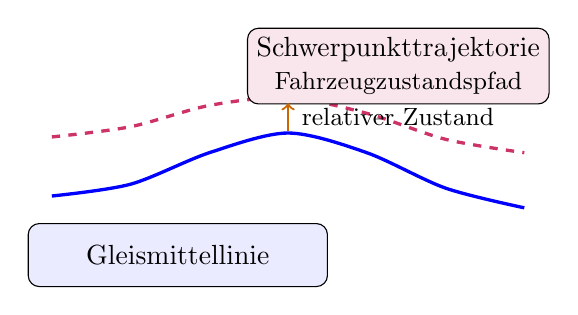
\begin{tikzpicture}[
  x=1cm,y=1cm,
  box/.style={draw, rounded corners, align=center, minimum width=3.8cm, minimum height=0.8cm}
]
\draw[very thick, blue] plot[smooth] coordinates {(0,0) (1,0.15) (2,0.55) (3,0.8) (4,0.55) (5,0.1) (6,-0.15)};
\draw[very thick, purple!80, dashed] plot[smooth] coordinates {(0,0.75) (1,0.88) (2,1.15) (3,1.25) (4,1.05) (5,0.72) (6,0.55)};

\node[box, fill=blue!8] at (1.6,-0.75) {Gleismittellinie};
\node[box, fill=purple!10] at (4.4,1.65) {Schwerpunkttrajektorie\\\small Fahrzeugzustandspfad};

\draw[->, thick, orange!80!black] (3,0.82) -- (3,1.18);
\node[right] at (3.05,1.0) {\small relativer Zustand};
\end{tikzpicture}

\caption{Trajektorie eines modellgewählten Bezugspunktes relativ zum Eisenbahnzustand; sie ist keine Alignment-Geometrie.}
\label{fig:schwerpunkt-trajectory}
\end{figure}

\begin{principle}[Qualifizierte Schwerpunktverwendung]
\label{princ:schwerpunkt-principle}
Jede Verwendung von \emph{Schwerpunkt} benennt zugehöriges Subjekt, Modell,
Bezugssystem und Evidenzstatus. Es handelt sich nicht um einen kanonischen
Kernel-Zustand.
\end{principle}

\begin{principle}[Schwerpunkt ist keine Geometrie]
\label{princ:schwerpunkt-not-geometry}
Die Änderung oder Bewertung einer Modellbezugspunkttrajektorie ändert weder
die Alignment Identity noch ersetzt sie die intrinsische Konstruktion.
\end{principle}

\section{Massenmittelpunkt und reduzierter Bezugspunkt}

Der physische Massenmittelpunkt ist eine Eigenschaft eines bestimmten
beladenen Fahrzeugs. Ein reduziertes Fahrzeugmodell \(M\) kann dagegen einen
Bezugspunkt \(P_M\) verwenden, der nur unter angegebenen Beladungs- und
Starrkörperannahmen mit einem angenommenen Massenmittelpunkt übereinstimmt.
Ein repräsentativer Trajektorienpunkt, ein Optimierungsaggregat und ein
begrifflicher Fokus sind andere Objekte und dürfen nicht stillschweigend
dasselbe Symbol erhalten.

\begin{definition}[Modellqualifizierter Bezugspunktzustand]
\label{def:cg-state}
Für das Fahrzeugsubjekt \(V\), das Antwortmodell \(M\), das Bezugssystem \(F\),
den qualifizierten Eisenbahnzustand \(S_{\mathrm{rail}}\), die Durchfahrt
\(s(t)\), Parameter \(Q_M\) und Anfangsbedingungen \(I_M\) ist
\[
x_{P_M}^{\mathrm{pred}}(t)
=
\mathcal D_M(S_{\mathrm{rail}}(s(t)),Q_M,I_M)_{{P_M},F}.
\]
Das Ergebnis ist eine Modellvorhersage mit Provenienz und Gültigkeit dieser
Eingaben. Es ist weder Beobachtung noch Nachweis der Bewegung des physischen
Massenmittelpunkts.
\end{definition}

\begin{definition}[Schwerpunkttrajektorie]
\label{def:cg-trajectory}
Die Schreibweise \(x_{\mathrm{CG}}(t)\) ist nur zulässig, wenn \(P_M\)
ausdrücklich als modellierter Massenmittelpunkt festgelegt wurde. Andernfalls
gilt \(x_{P_M}(t)\).
\end{definition}

\section{Was abgeleitet werden darf}

\begin{definition}[Operatives Gleichgewicht]
\label{def:operational-balance}
Operatives Gleichgewicht bezeichnet hier eine erklärte Modellrelation in
einem erklärten Bezugssystem, keinen allgemeinen Fahrzeugzustand.
\end{definition}

\begin{definition}[Gleichgewichtstrajektorie]
\label{def:balance-trajectory}
Eine Gleichgewichtstrajektorie ist das zeit- oder stationsabhängige Ergebnis
dieser Relation einschließlich Modell, Frame, Vorzeichen-, Geschwindigkeits-
und Überhöhungsannahmen.
\end{definition}

\begin{definition}[Effektive operative Beschleunigung]
\label{def:effective-operational-acceleration}
Im reduzierten Gleis-Frame-Test aus \cref{chap:dynamic-balance} ist
\(a_{\mathrm{eff}}=v^2\kappa-g\sin\phi\) ein Residuenindikator. Es ist nicht
die Beschleunigung von \(P_M\), solange kein Antwortmodell diese Abbildung
begründet.
\end{definition}

\begin{definition}[Rollentwicklung]
\label{def:roll-evolution}
Rollentwicklung ist eine Ausgabe eines Antwortmodells und benötigt Trägheit,
Federung, Beladung, Anfangsbedingungen und Frame-Konvention; Überhöhung allein
bestimmt sie nicht.
\end{definition}

\begin{definition}[Operativer Komfort]
\label{def:operational-comfort}
Komfort ist eine zweck- und regelqualifizierte Bewertung anwendbarer Evidenz.
Weder Bezugspunkttrajektorie noch reduziertes Gleichgewichtsresiduum sind
allein eine Komfortaussage.
\end{definition}

\begin{definition}[Operative Trajektorienformung]
\label{def:trajectory-shaping}
Trajektorienformung bezeichnet erst dann eine Optimierung, wenn Variablen,
Nebenbedingungen, Antwortmodell und Ziel erklärt sind. Ihr Ergebnis ist ein
Kandidat.
\end{definition}

\section{Schwerpunktinterpretation und Realisierung}

Soll-Alignment, Metric Realization, gebautes Asset, beobachtete
Zustandsschätzung und vorhergesagte Bezugspunktantwort bleiben getrennt. Ein
Modell darf eine qualifizierte Realisierung oder beobachtete Zustandsschätzung
verwenden; seine Ausgabe erbt deren Unsicherheit und Anwendbarkeit. Der
Ausdruck \emph{Schwerpunkt-Trassierung} ist daher historische oder
illustrative Kurzform für eine modellqualifizierte Untersuchung der
Bezugspunkttrajektorie. Er bezeichnet weder einen Kernel-Begriff noch eine
aktuelle AXTRAN-Fähigkeit.

\section{Aussagestatus}

\begin{center}
\small
\begin{tabular}{p{0.28\linewidth}p{0.25\linewidth}p{0.38\linewidth}}
\toprule
Ausdruck & Status & Vertretbare Verwendung\\
\midrule
physischer Massenmittelpunkt & physischer/Modellparameter & bestimmtes Fahrzeug und Beladung\\
\(P_M\)-Trajektorie & Modellvorhersage & identifizierte \(M,F,Q_M,I_M\)\\
Schwerpunktzustand & nichtkanonische Kurzform & nur mit vorstehender Qualifikation\\
Schwerpunktoptimierung & Kandidat & nur für erklärtes Optimierungsproblem\\
\bottomrule
\end{tabular}
\end{center}

Das nächste Kapitel verwendet bewusst die einfachste Residuenrelation. Ihre
Grenzen zeigen, warum eine Modellausgabe nicht durch einen zustandsähnlichen
Namen zur Bewertung oder Entscheidung wird.
